\chapter{\ifproject%
      \ifenglish Project Structure and Methodology\else โครงสร้างและขั้นตอนการทำงาน\fi
  \else%
      \ifenglish Project Structure\else โครงสร้างของโครงงาน\fi
  \fi
 }

ในบทนี้จะกล่าวถึงหลักการ และการออกแบบระบบ

\makeatletter

% \renewcommand\section{\@startsection {section}{1}{\z@}%
%                                    {13.5ex \@plus -1ex \@minus -.2ex}%
%                                    {2.3ex \@plus.2ex}%
%                                    {\normalfont\large\bfseries}}

\makeatother
%\vspace{2ex}
% \titleformat{\section}{\normalfont\bfseries}{\thesection}{1em}{}
% \titlespacing*{\section}{0pt}{10ex}{0pt}

\section{หลักการทำงานของระบบ}


% \begin{figure}
% \begin{center}
% \includegraphics{800px-Briny_Beach.jpg}
% \end{center}
% \caption[Poem]{The Walrus and the Carpenter}
% \label{fig:walrus}
% \end{figure}
\subsection{การทำงานของระบบ (System Architecture)}
\begin{figure}[h]
    \begin{center}
        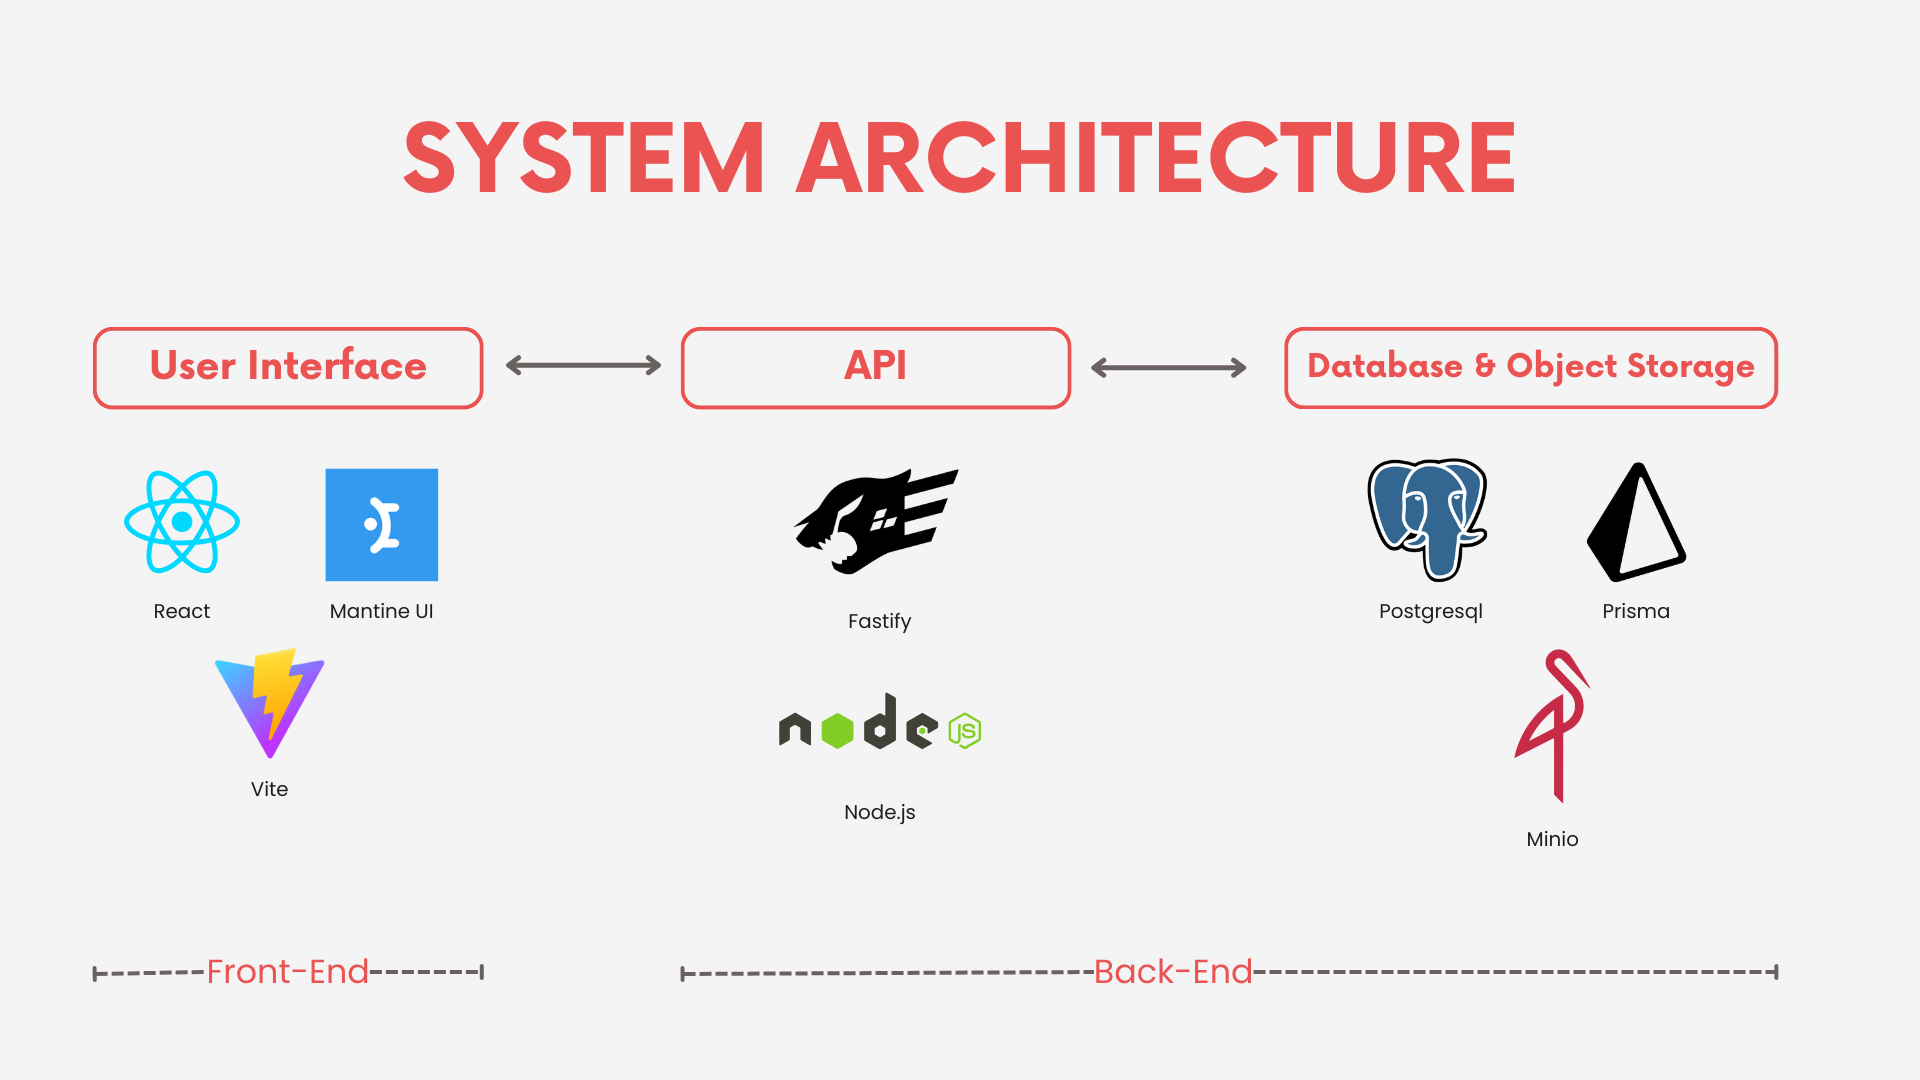
\includegraphics[width=0.9\textwidth]{img/system achitecture.png}
    \end{center}
    \caption[Poem]{System Architecture}
    \label{fig:system_overview}
\end{figure}

จากรูปที่ \ref{fig:system_overview} จะเป็นภาพรวมของระบบที่เราได้ทำการออกแบบขึ้น โดยมีรายละเอียดดังนี้
\begin{itemize}
    \item Frontend

          ส่วนหน้าบ้าน (Frontend) เป็นส่วนการพัฒนาเพื่อแสดง User Interface (UI) โดยโครงการนี้ได้ใช้เทคโนโลยี React ร่วมกับ Mantine UI ในการออกแบบและสร้างส่วนติดต่อผู้ใช้ (UI) โดยมีหน้าที่แสดงผลลัพธ์ต่อผู้ใช้ในรูปแบบที่เข้าใจง่าย รับข้อมูลป้อนจากผู้ใช้ผ่านอินเทอร์เฟซต่าง ๆ เช่น ปุ่ม ฟิลด์ข้อความ ฯลฯ และสื่อสารกับ API เพื่อส่งคำร้องขอและรับผลลัพธ์
    \item Backend

          ส่วนหลังบ้าน (Backend) เป็นส่วนที่ทำหน้าที่รับข้อมูลจากผู้ใช้ จากนั้นทำการประมวลผลข้อมูล และส่งข้อมูลกลับไปยังผู้ใช้ โดยโครงการนี้ได้ใช้เทคโนโลยี Fastify เว็บเฟรมเวิร์ค Node.js ร่วมกับ Prisma ORM ในการจัดการข้อมูลในฐานข้อมูล รวมถึงทำการสื่อสารกับฐานข้อมูล PostgreSQL และ Minio (Object Storage) ในการจัดการข้อมูลที่เป็นไฟล์
\end{itemize}

\subsection{เส้นทางของผู้ใช้ (User Flow)}
\begin{figure}[h]
    \begin{center}
        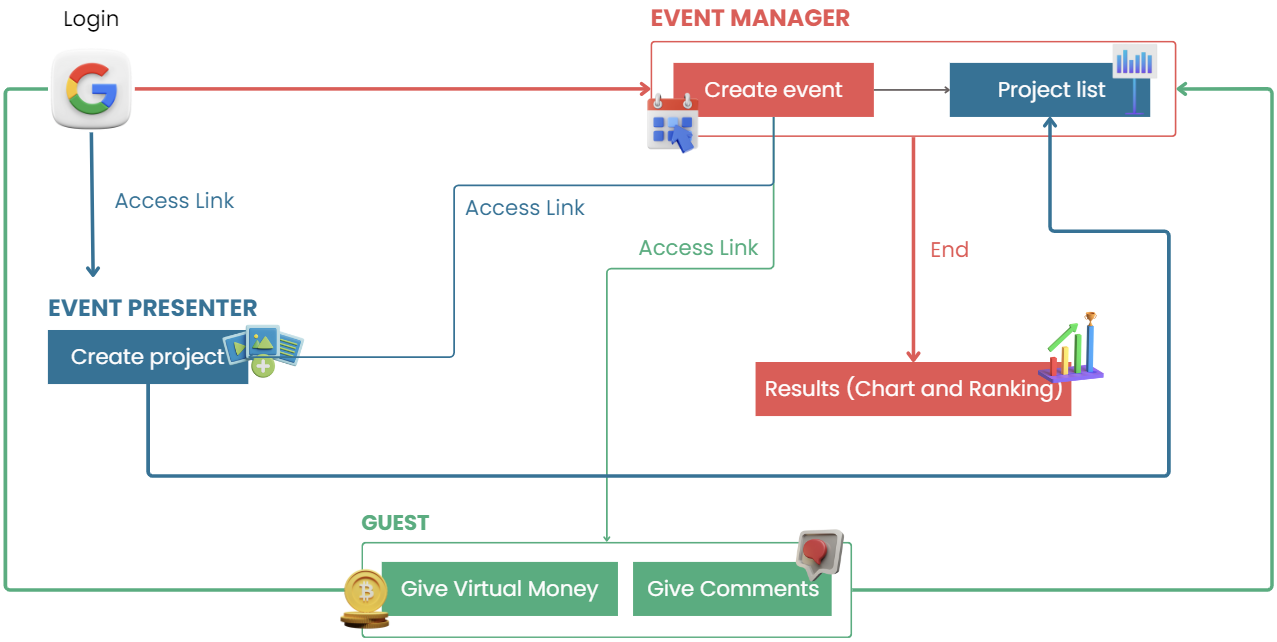
\includegraphics[width=0.9\textwidth]{img/userflow.png}
    \end{center}
    \caption[Poem]{User Flow}
    \label{fig:user_flow}
\end{figure}

จากรูปที่ \ref{fig:user_flow} จะเป็นเส้นทางของผู้ใช้งานที่เข้าใช้งานระบบ โดยมีรายละเอียดดังนี้

\subsubsection{ผู้สร้างงานกิจกรรม (Event Manager)}
\begin{itemize}
    \item ผู้ใช้เข้าสู่ระบบโดยใช้ Google Account
    \item ผู้ใช้สร้าง Event ใหม่ โดยป้อนข้อมูลต่างๆ เช่น ชื่องานกิจกรรม รายละเอียด วันเวลา สถานที่ เป็นต้น
    \item ผู้ใช้สร้าง Event เสร็จสิ้น จะมี QR Code หรือ Access Link สำหรับนำไปให้ผู้นำเสนอโครงการ (Presenter) สำหรับเพิ่มโครงการของตนและผู้เข้าร่วมกิจกรรม (Guest) สำหรับเข้าร่วมกิจกรรม
    \item ผู้ใช้สามารถดูผลลัพธ์ (Chart และ Ranking) ของโครงการต่าง ๆ ที่เข้าร่วมกิจกรรมในระหว่างจัดงานกิจกรรม

\end{itemize}

\subsubsection{ผู้นำเสนอโครงการ (Presenter)}
\begin{itemize}
    \item ผู้ใช้เข้าสู่ระบบโดยใช้ Google Account
    \item ผู้ใช้สร้าง Project ใหม่ โดยป้อนข้อมูลต่าง ๆ เช่น ชื่อโครงการ รายละเอียด รูปภาพ ลิงก์ และไฟล์อื่น ๆ ที่เกี่ยวข้อง
    \item ผู้ใช้ดูผลลัพธ์ว่าโครงการของตนได้รับ Virtual Money จากผู้เข้าร่วมกิจกรรม (Guest) และความคิดเห็นเกี่ยวกับโครงการของตนหลังจากเสร็จสิ้นงานกิจกรรม

\end{itemize}

\subsubsection{ผู้เข้าร่วมกิจกรรม (Guest)}
\begin{itemize}
    \item ผู้ใช้เข้าร่วม Event โดยใช้ QR COde หรือ Access Link ที่ได้รับจาก Event Manager
    \item ผู้ใช้เข้าสู่ระบบโดยใช้ Google Account
    \item ผู้ใช้ดูรายละเอียดของงานกิจกรรมที่จัดขึ้น รวมถึงโครงการที่เข้าร่วมกิจกรรม
    \item ผู้ใช้สามารถให้ Virtual Money และแสดงความคิดเห็นเกี่ยวกับ Project ต่าง ๆ ที่เข้าร่วมกิจกรรมได้
\end{itemize}

\subsection{โครงสร้างฐานข้อมูล (Database Schema)}
\begin{figure}[h]
    \begin{center}
        \includegraphics[width=0.9\textwidth]{img/database schama.png}
    \end{center}
    \caption[Poem]{Database Schema}
    \label{fig:data_schema}
\end{figure}
จากรูปที่ \ref{fig:data_schema} จะเป็นโครงสร้างของฐานข้อมูลที่ใช้ในระบบ โดยมีรายละเอียดดังนี้


\section{ส่วนเชื่อมต่อระหว่างผู้ใช้งานกับระบบ (User Interface)}
\subsection{ผู้ใช้งาน (User)}
\subsubsection{หน้าเข้าสู่ระบบ (Login Page)}
\begin{figure}[h]
    \begin{center}
        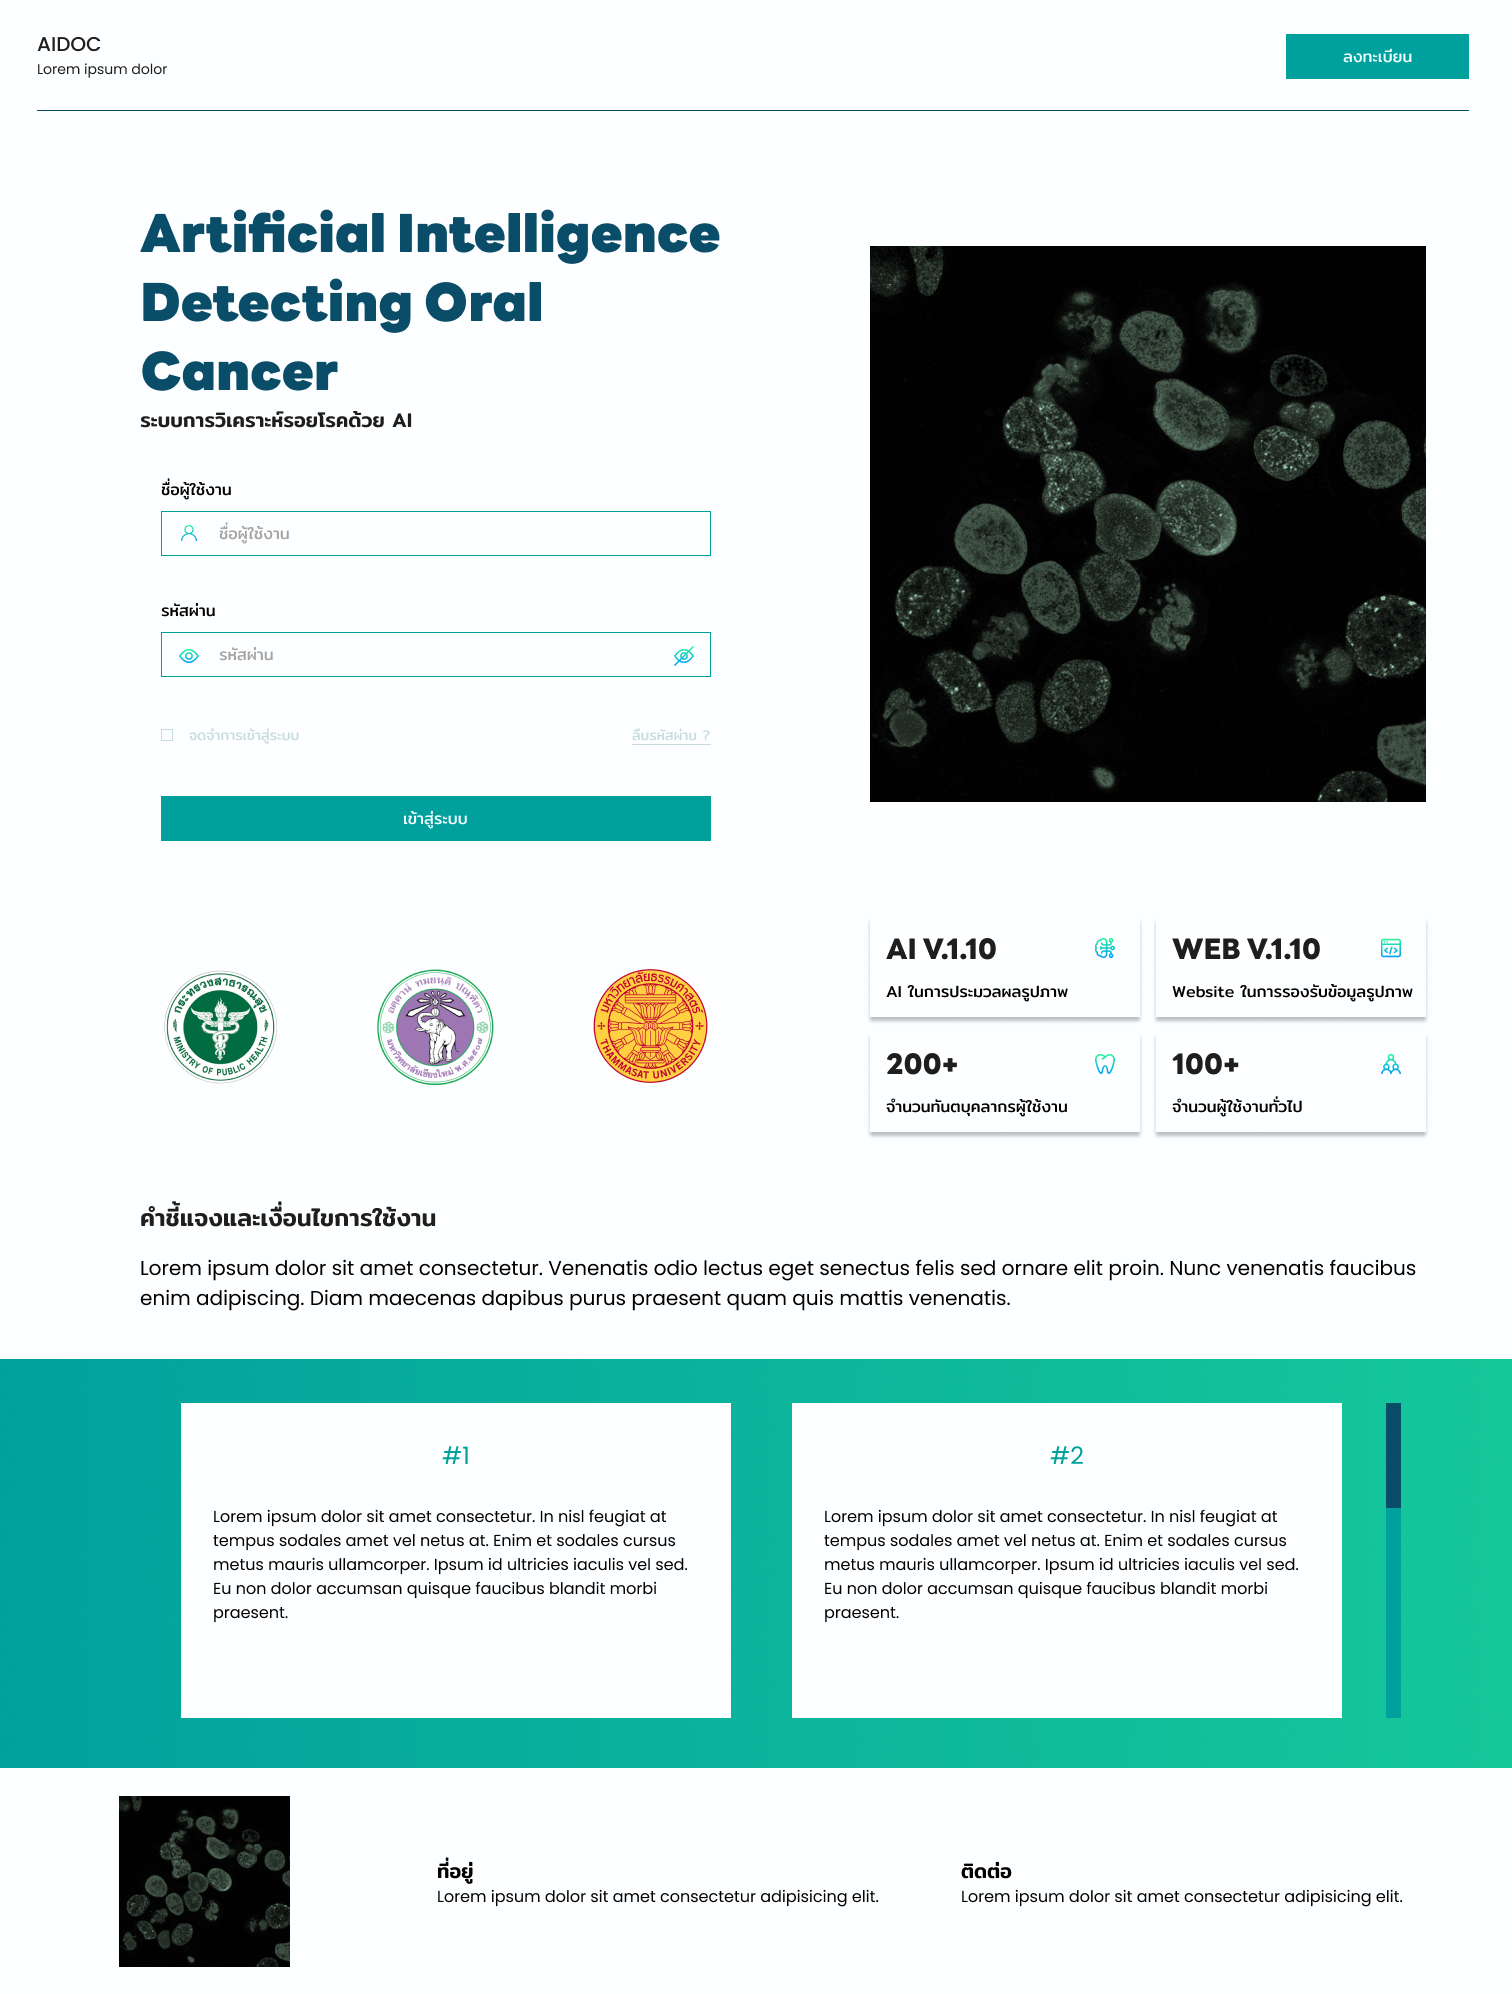
\includegraphics[width=0.7\textwidth]{img/user/1-login-page.png}
    \end{center}
    \caption[Poem]{Login Page}
    \label{fig:login}
\end{figure}

\newpage
\subsubsection{หน้าลงทะเบียน (Register Page)}
\begin{figure}[h]
    \begin{center}
        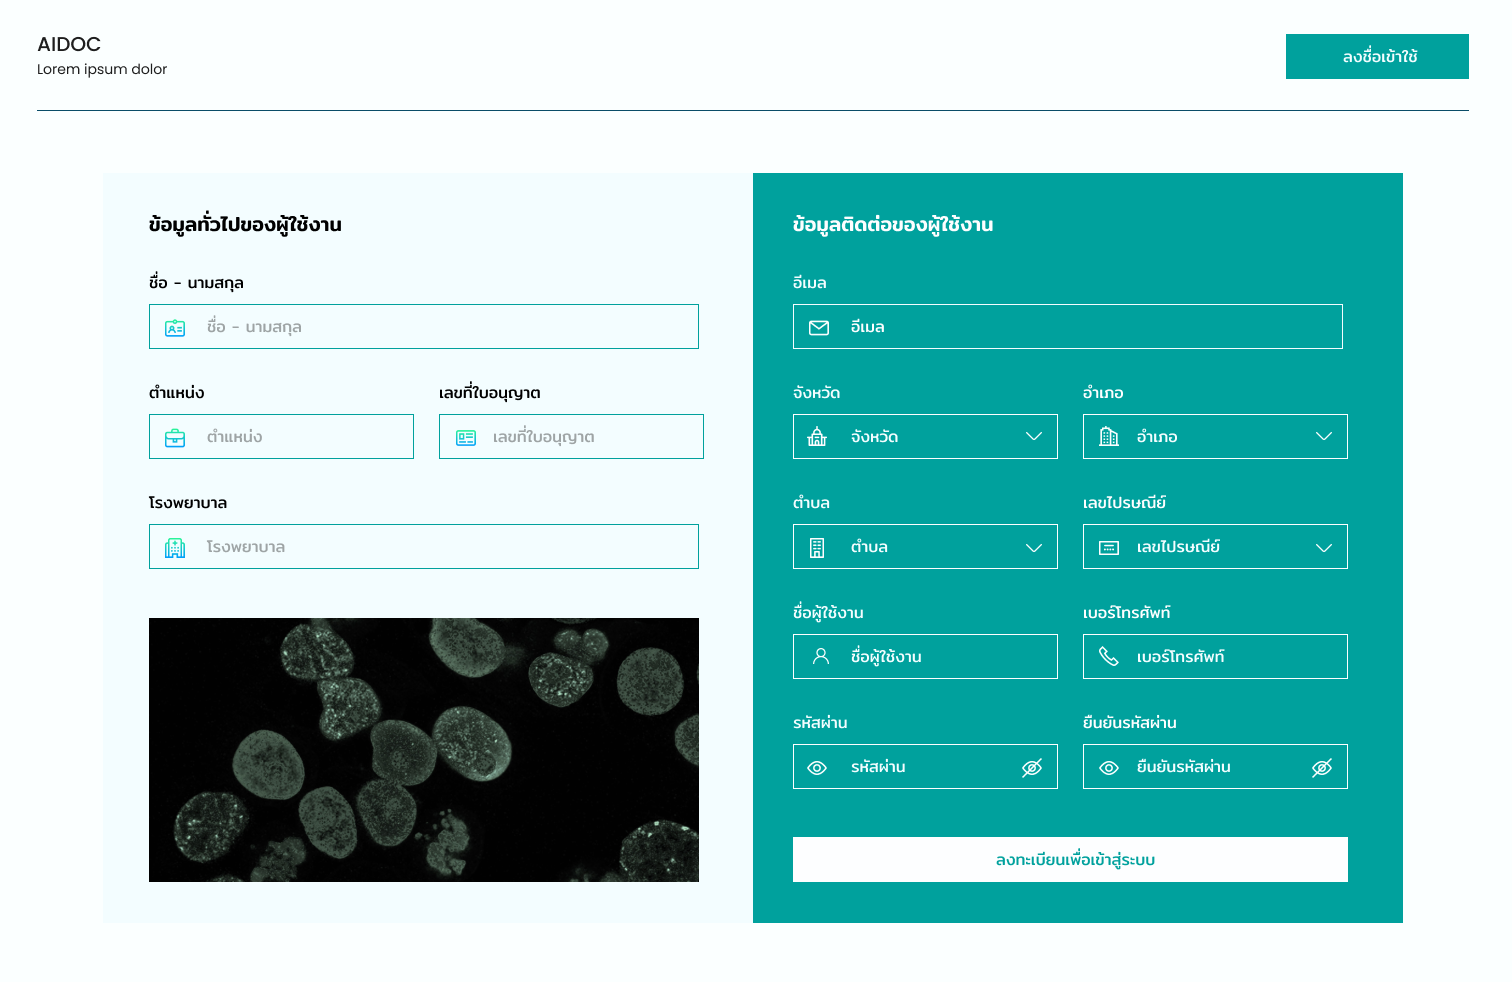
\includegraphics[width=0.7\textwidth]{img/user/2-register-page.png}
    \end{center}
    \caption[Poem]{Register Page}
    \label{fig:register}
\end{figure}

\subsubsection{หน้าประวัติการอัพโหลดรูปภาพ (History Page)}
\begin{figure}[h]
    \begin{center}
        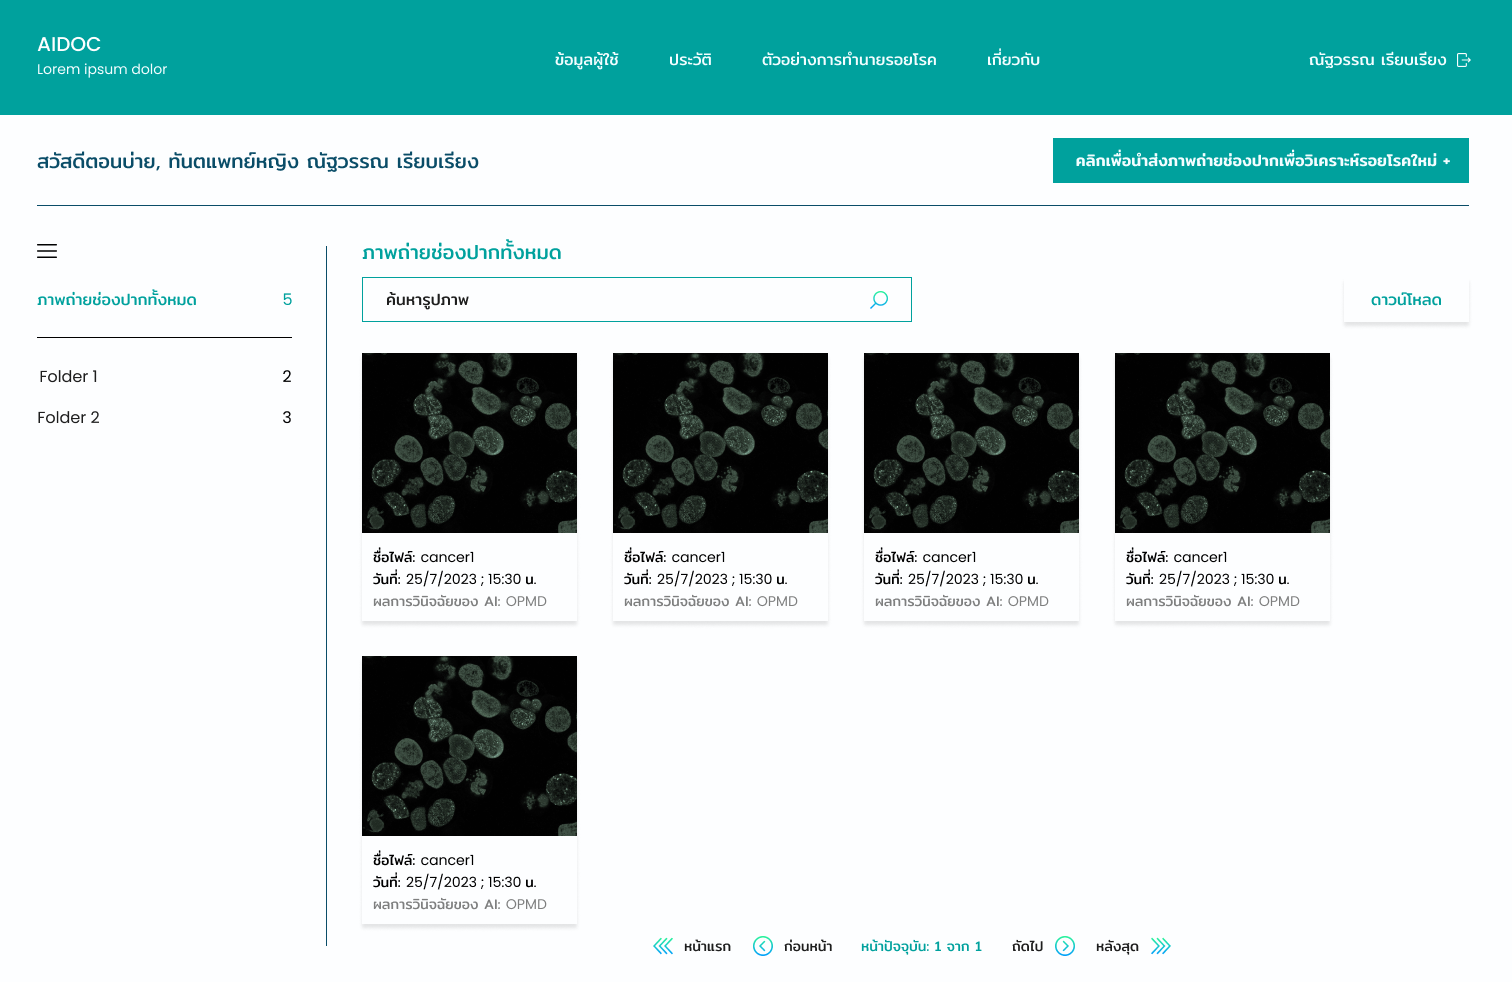
\includegraphics[width=0.7\textwidth]{img/user/3-1-histort-page.png}
    \end{center}
    \caption[Poem]{History Page}
    \label{fig:history}
\end{figure}

\begin{figure}[h]
    \begin{center}
        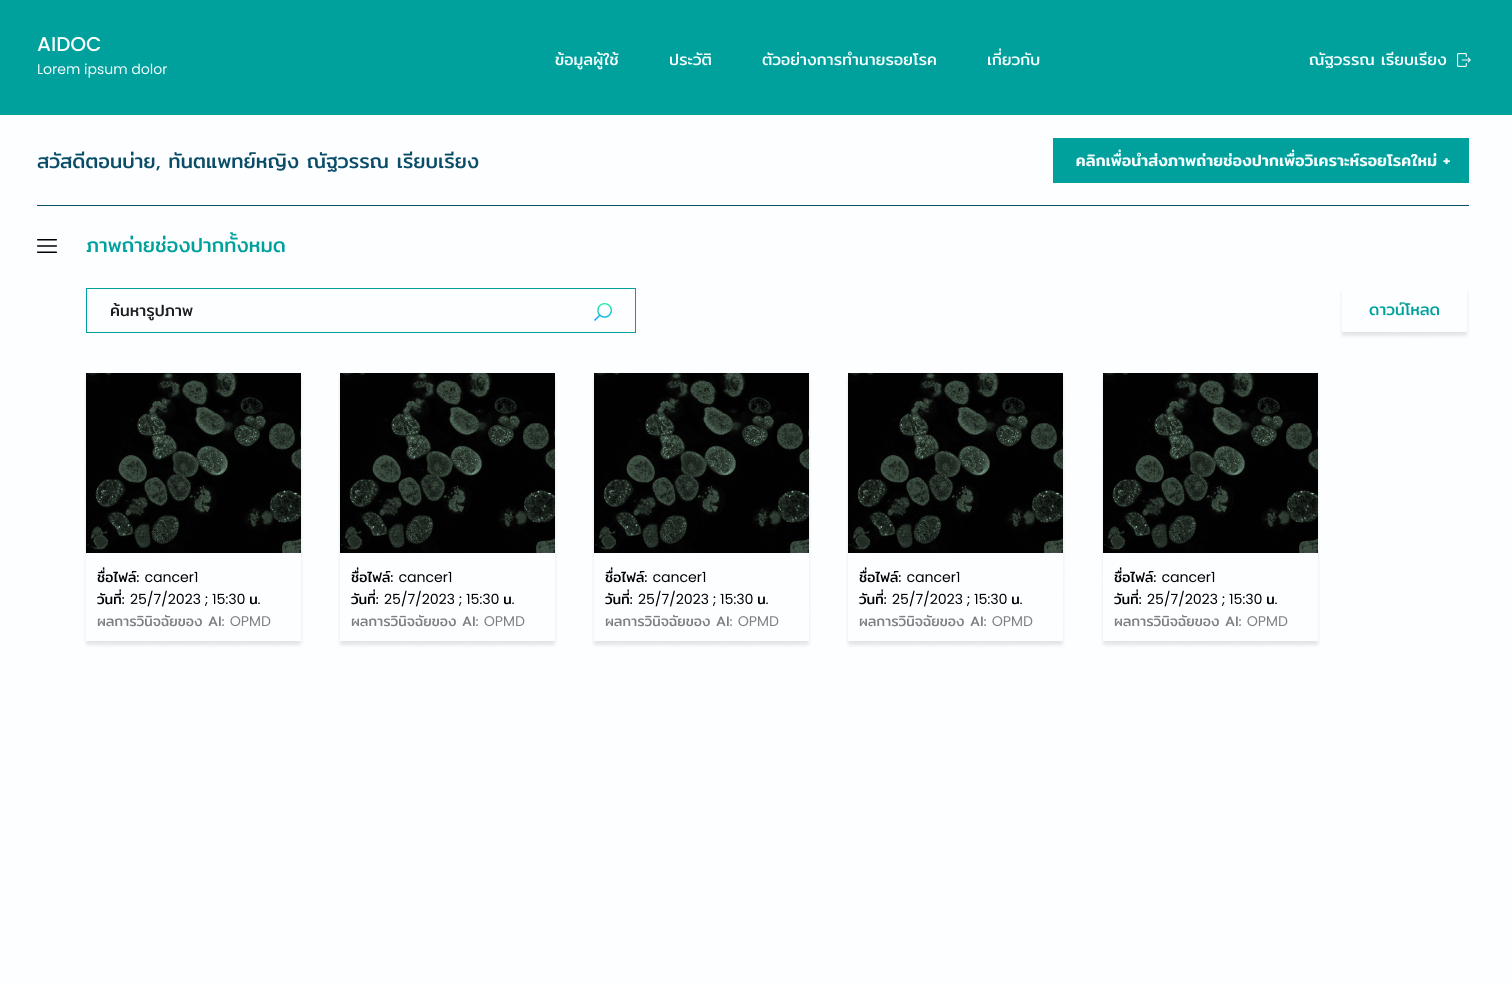
\includegraphics[width=0.7\textwidth]{img/user/3-histort-page.png}
    \end{center}
    \caption[Poem]{History Page}
    \label{fig:history_2}
\end{figure}

\newpage
\subsubsection{หน้าอัพโหลดรูปภาพ (Upload Page)}
\begin{figure}[h]
    \begin{center}
        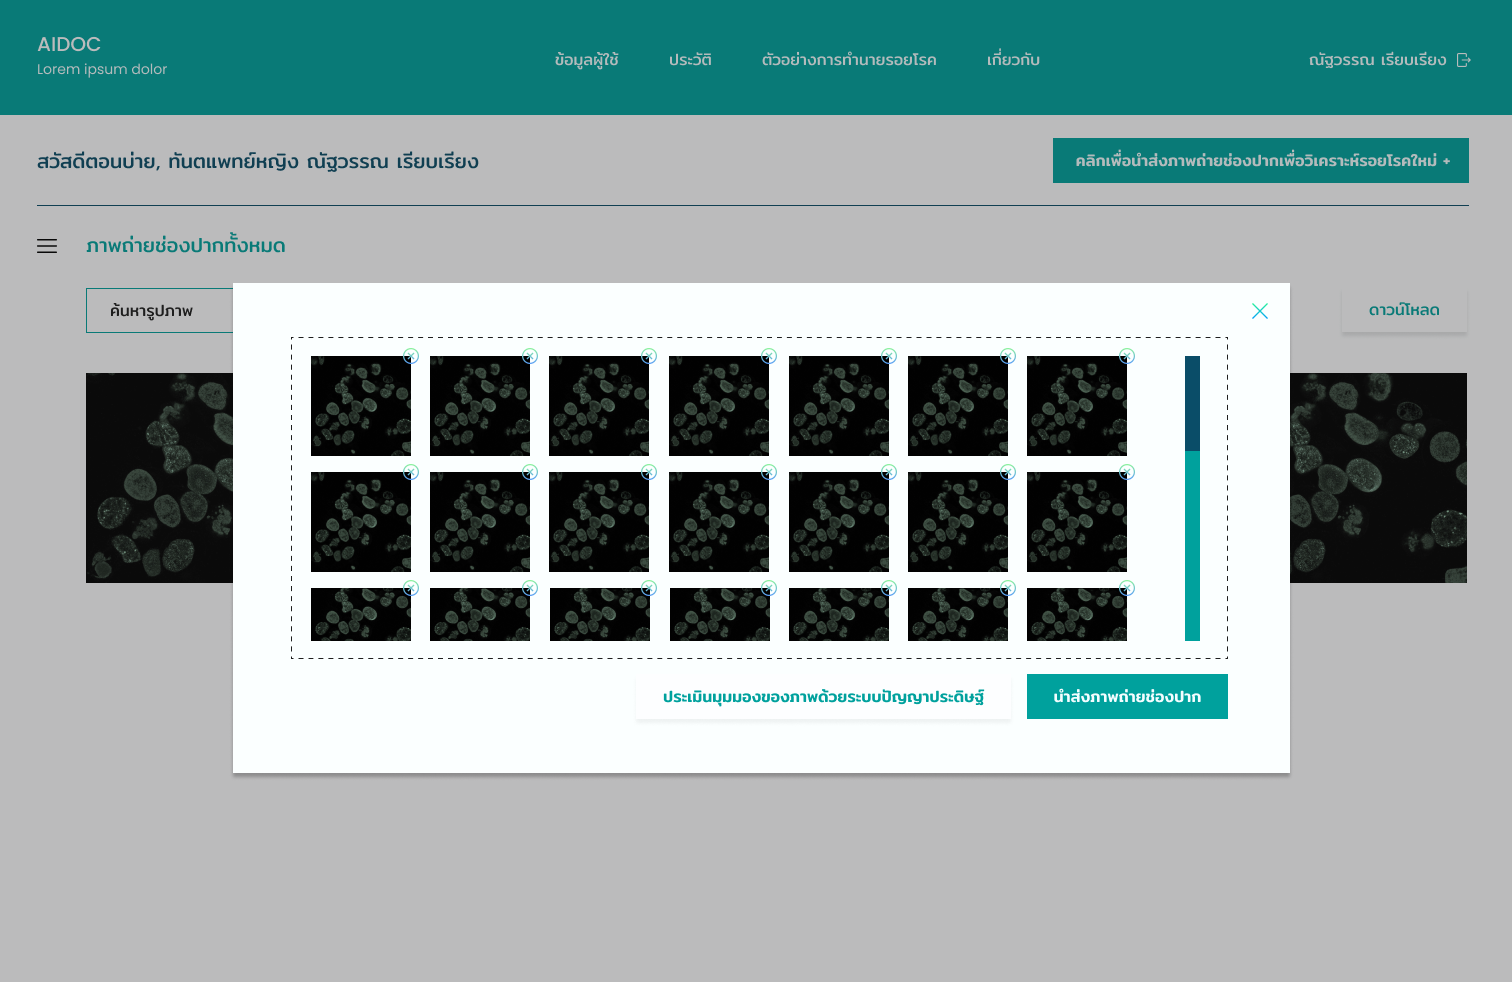
\includegraphics[width=0.7\textwidth]{img/user/4-1-upload-image-pop-up.png}
    \end{center}
    \caption[Poem]{Upload Page}
    \label{fig:upload}
\end{figure}

\begin{figure}[h]
    \begin{center}
        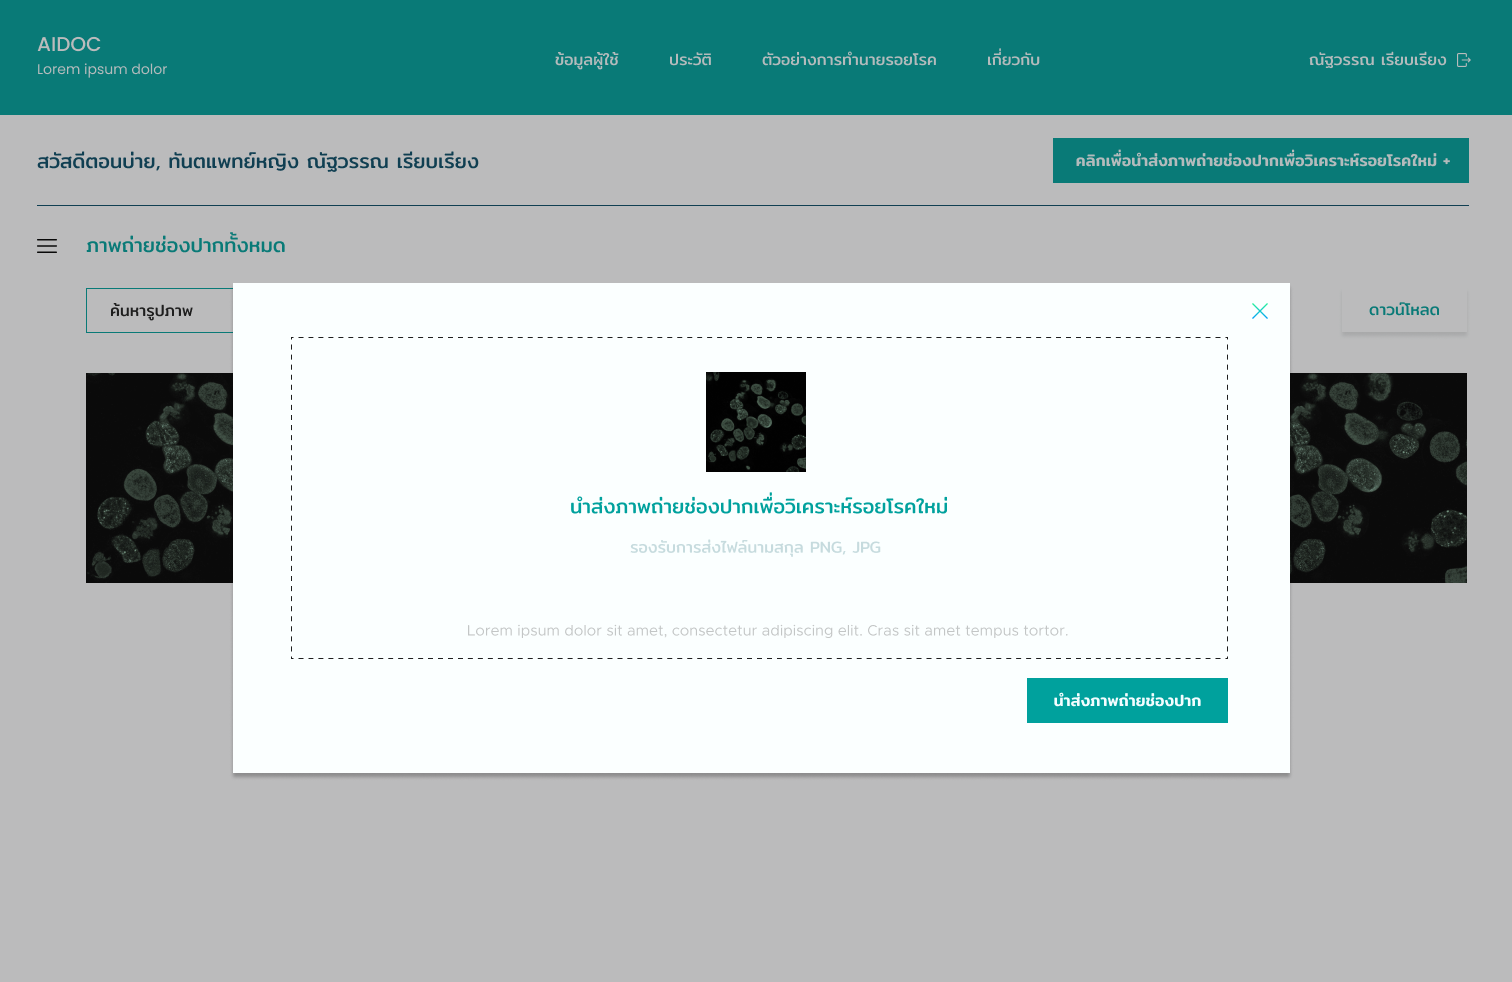
\includegraphics[width=0.7\textwidth]{img/user/4-upload-image-pop-up.png}
    \end{center}
    \caption[Poem]{Upload Page}
    \label{fig:upload_2}
\end{figure}

\newpage
\subsubsection{หน้าแสดงผลการทำนายรอยโรคในช่องปาก (Result Page)}
\begin{figure}[h]
    \begin{center}
        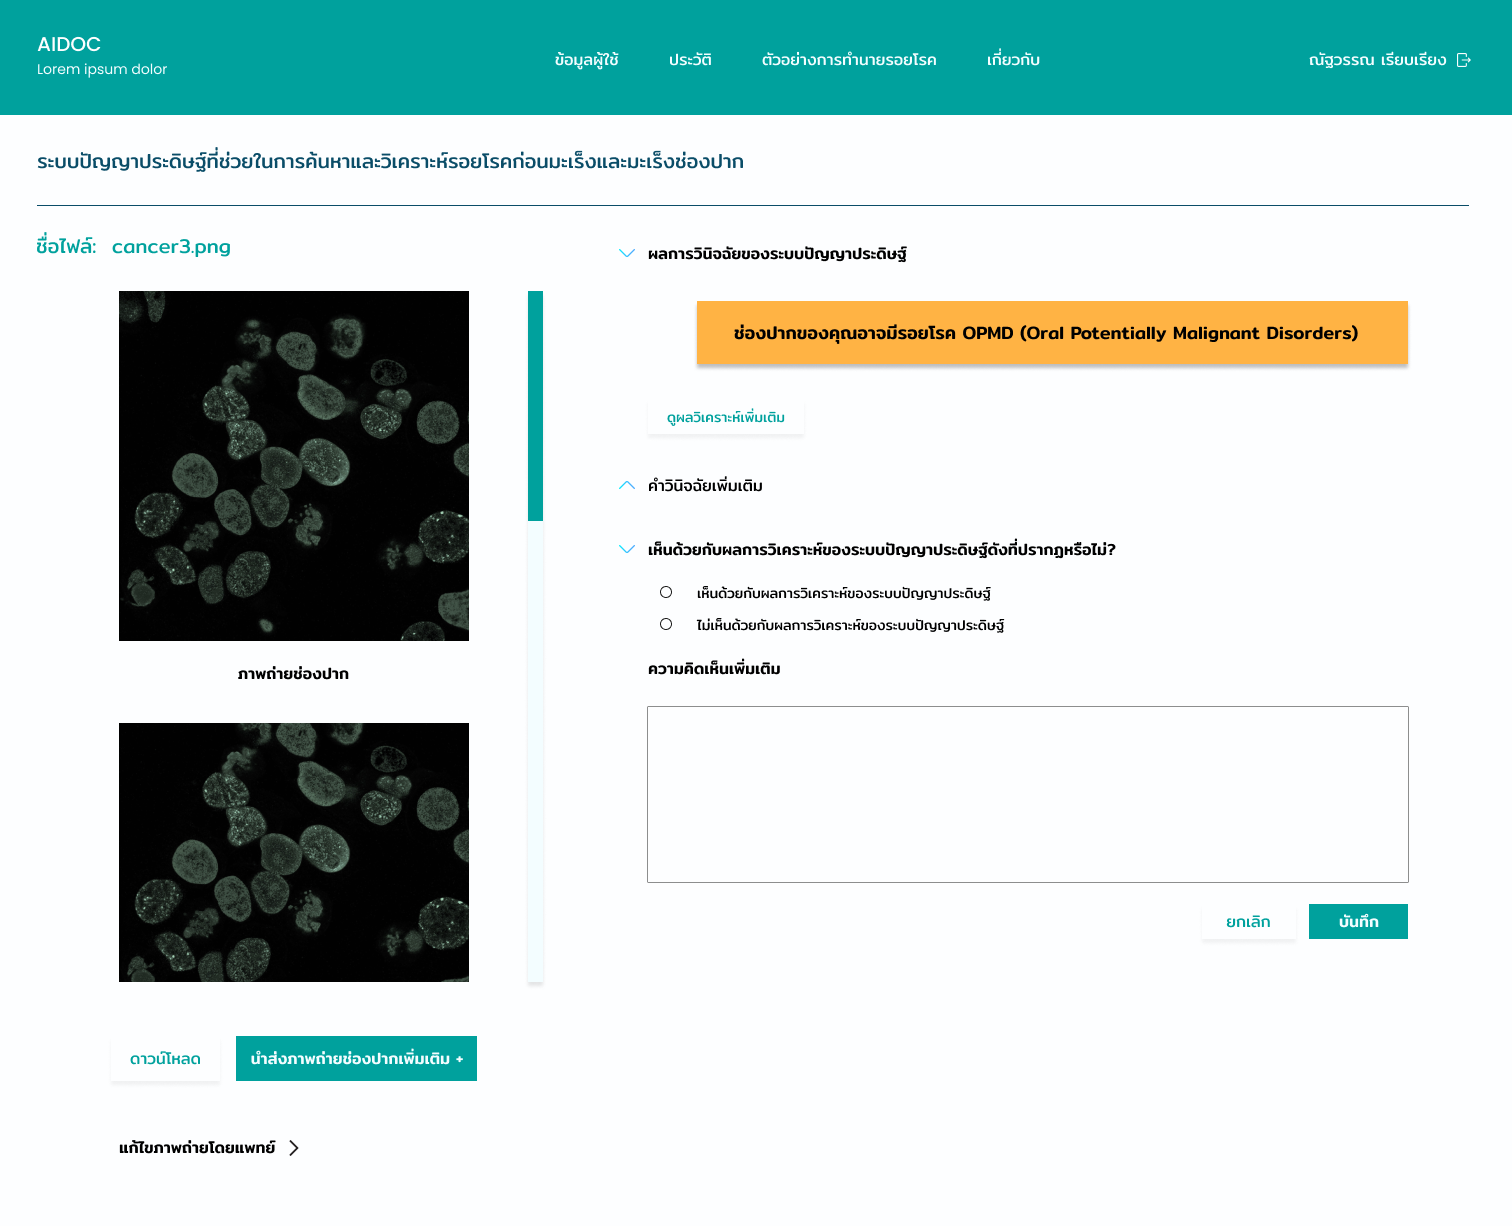
\includegraphics[width=0.7\textwidth]{img/user/predictionPage-5.png}
    \end{center}
    \caption[Poem]{Result Page}
    \label{fig:result}
\end{figure}

\newpage
\subsubsection{หน้าสำหรับวงรอยโรคในช่องปาก (Annotation Page)}
\begin{figure}[h]
    \begin{center}
        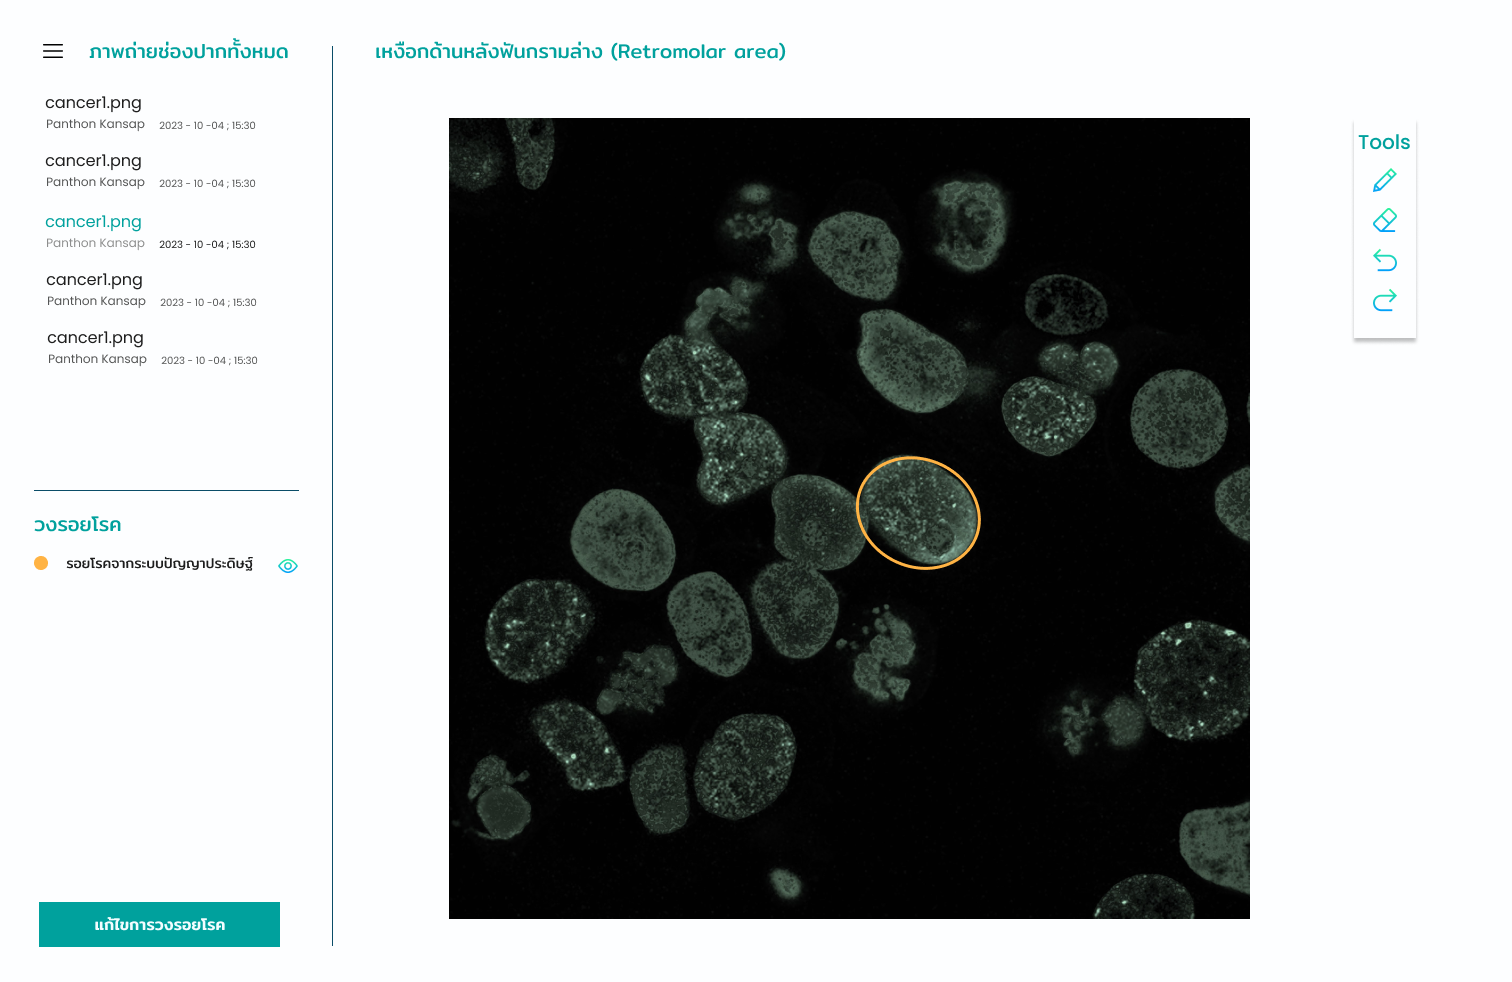
\includegraphics[width=0.7\textwidth]{img/user/6-annotation-page.png}
    \end{center}
    \caption[Poem]{Annotation Page}
    \label{fig:annotation}
\end{figure}

\subsubsection{หน้าแก้ไขข้อมูลส่วนตัว (Edit Profile Page)}
\begin{figure}[h]
    \begin{center}
        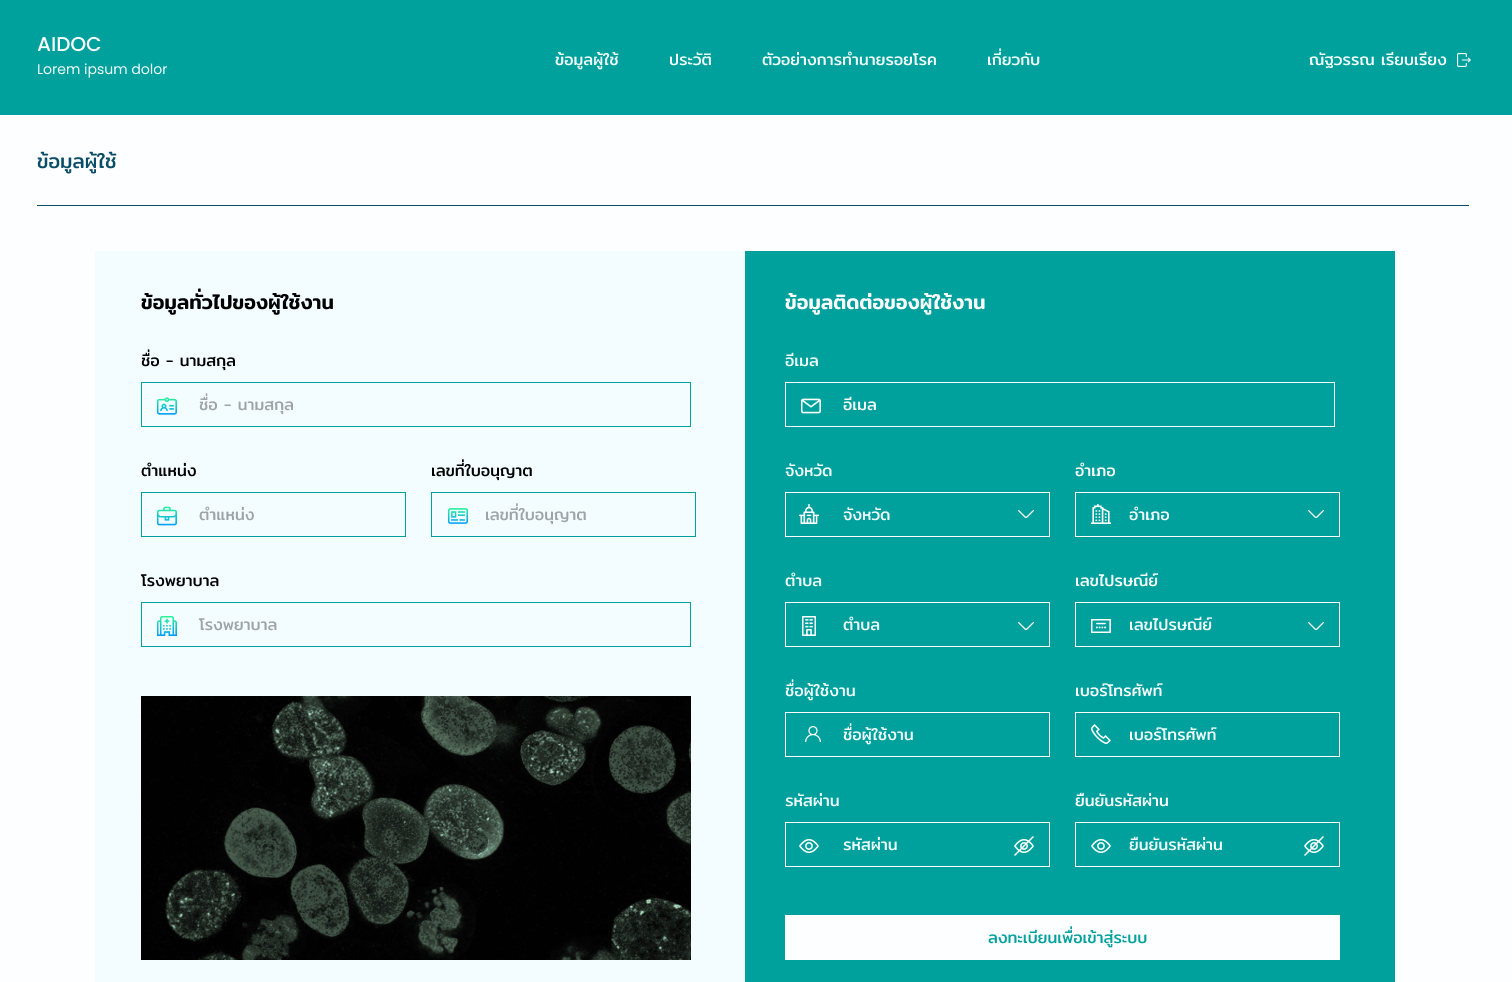
\includegraphics[width=0.7\textwidth]{img/user/7-user-management-page.png}
    \end{center}
    \caption[Poem]{Edit Profile Page}
    \label{fig:edit_profile}
\end{figure}


\newpage
\subsection{ผู้ดูแลระบบ (Admin)}

\subsubsection{หน้าอัพโหลดรูปภาพทั้งหมด (Upload Page)}
\begin{figure}[h]
    \begin{center}
        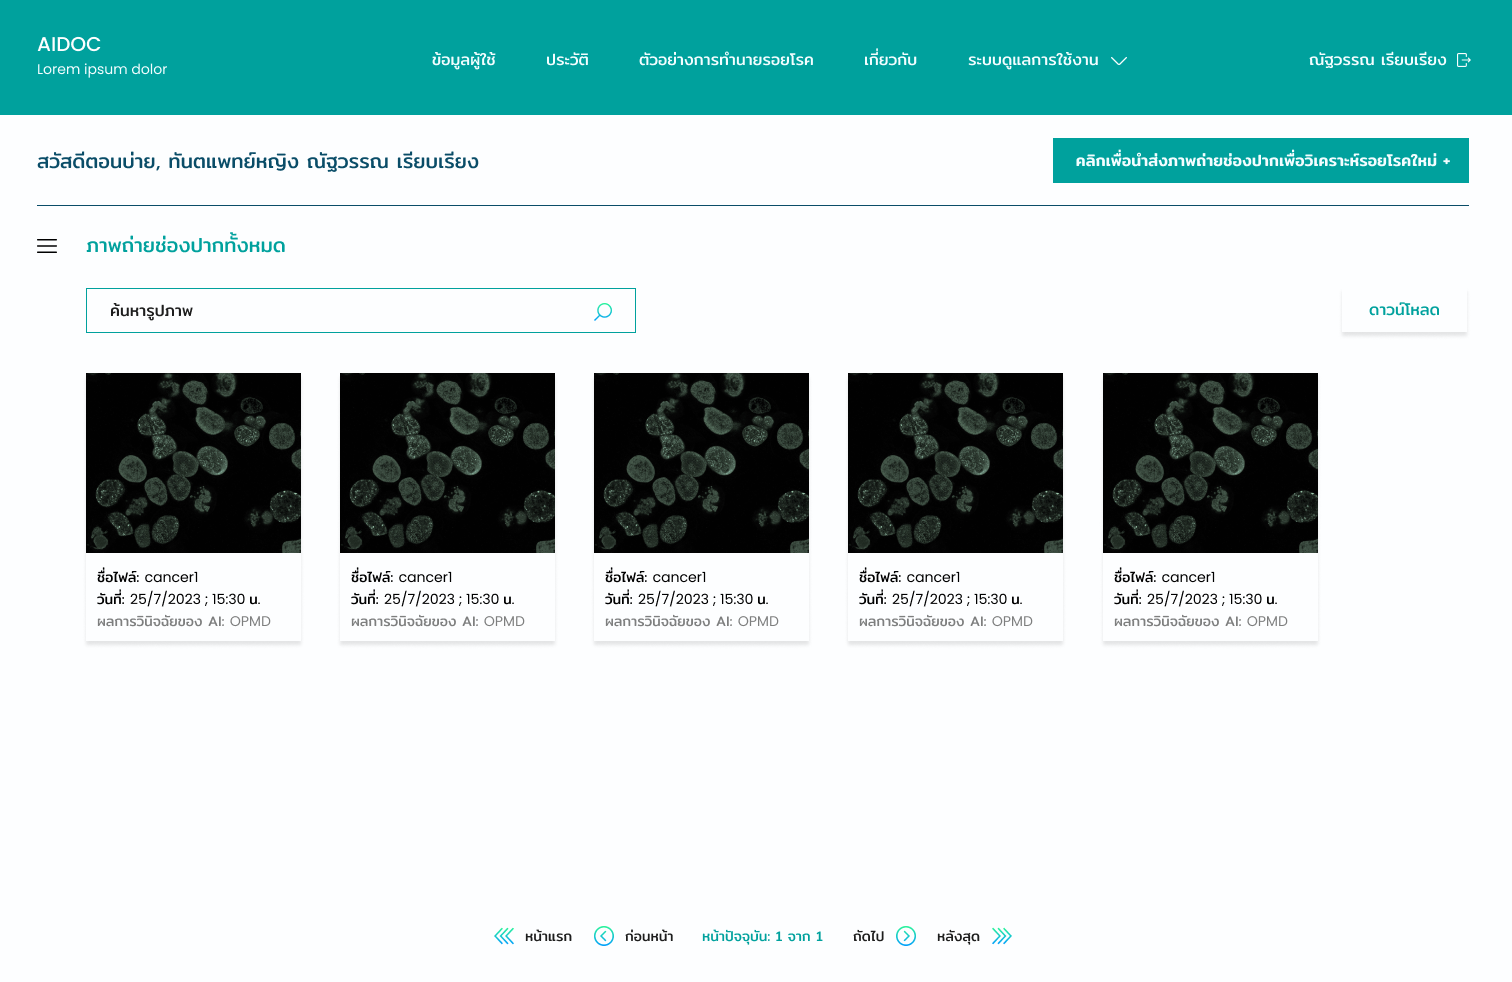
\includegraphics[width=0.7\textwidth]{img/admin/1-admin-historyPage.png}
    \end{center}
    \caption[Poem]{Upload Page}
    \label{fig:admin_upload}
\end{figure}


\subsubsection{หน้าจัดการผู้ใช้งาน (User Management Page)}
\begin{figure}[h]
    \begin{center}
        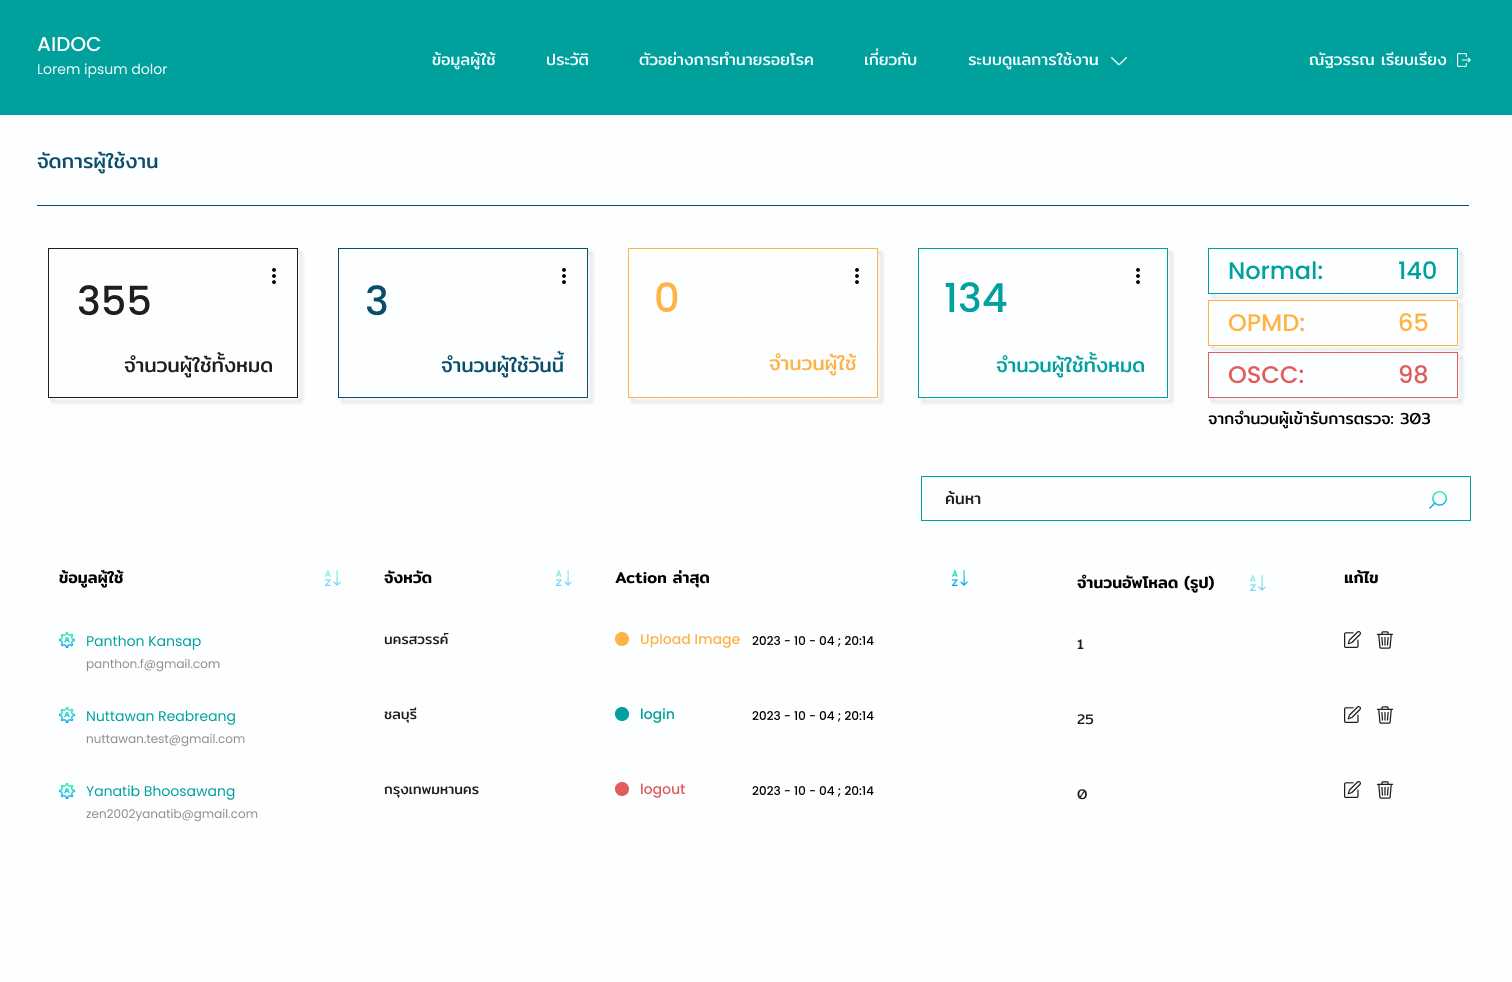
\includegraphics[width=0.7\textwidth]{img/admin/2-admin-user-management-page.png}
    \end{center}
    \caption[Poem]{User Management Page}
    \label{fig:user_management}
\end{figure}

\newpage
\subsubsection{หน้าจัดการข้อมูล (Data Management Page)}
\begin{figure}[h]
    \begin{center}
        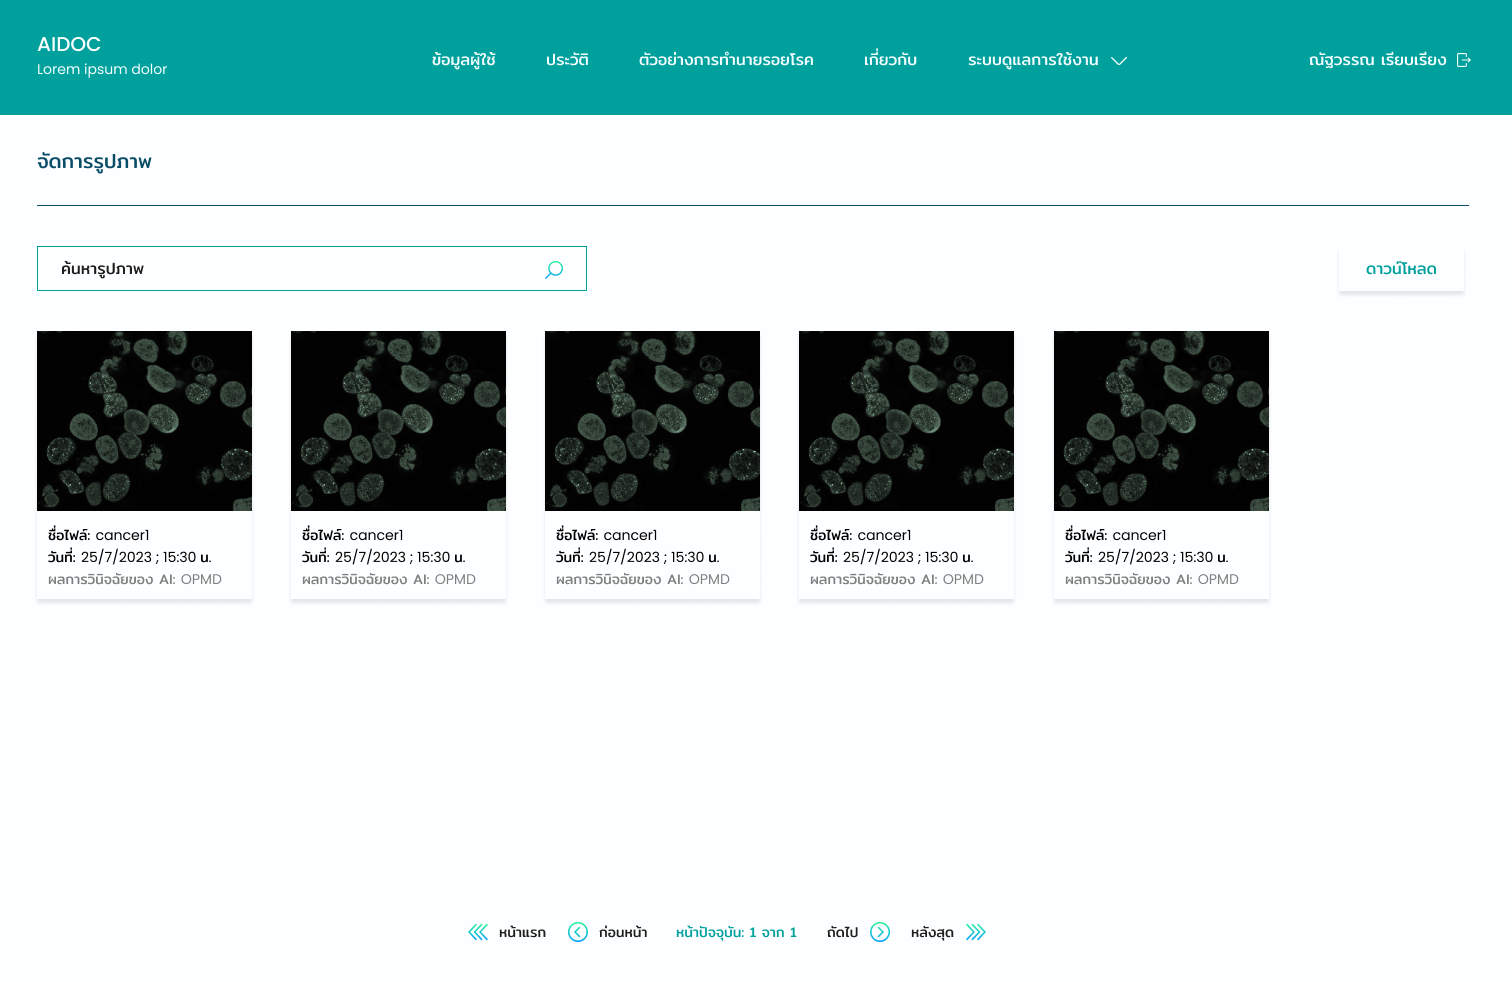
\includegraphics[width=0.7\textwidth]{img/admin/3-admin-image-manamgement.png}
    \end{center}
    \caption[Poem]{Data Management Page}
    \label{fig:data_management}
\end{figure}

\subsubsection{หน้าจัดการข้อมูล (Data Management Page) โดยแยกตามผู้ใช้งาน}
\begin{figure}[h]
    \begin{center}
        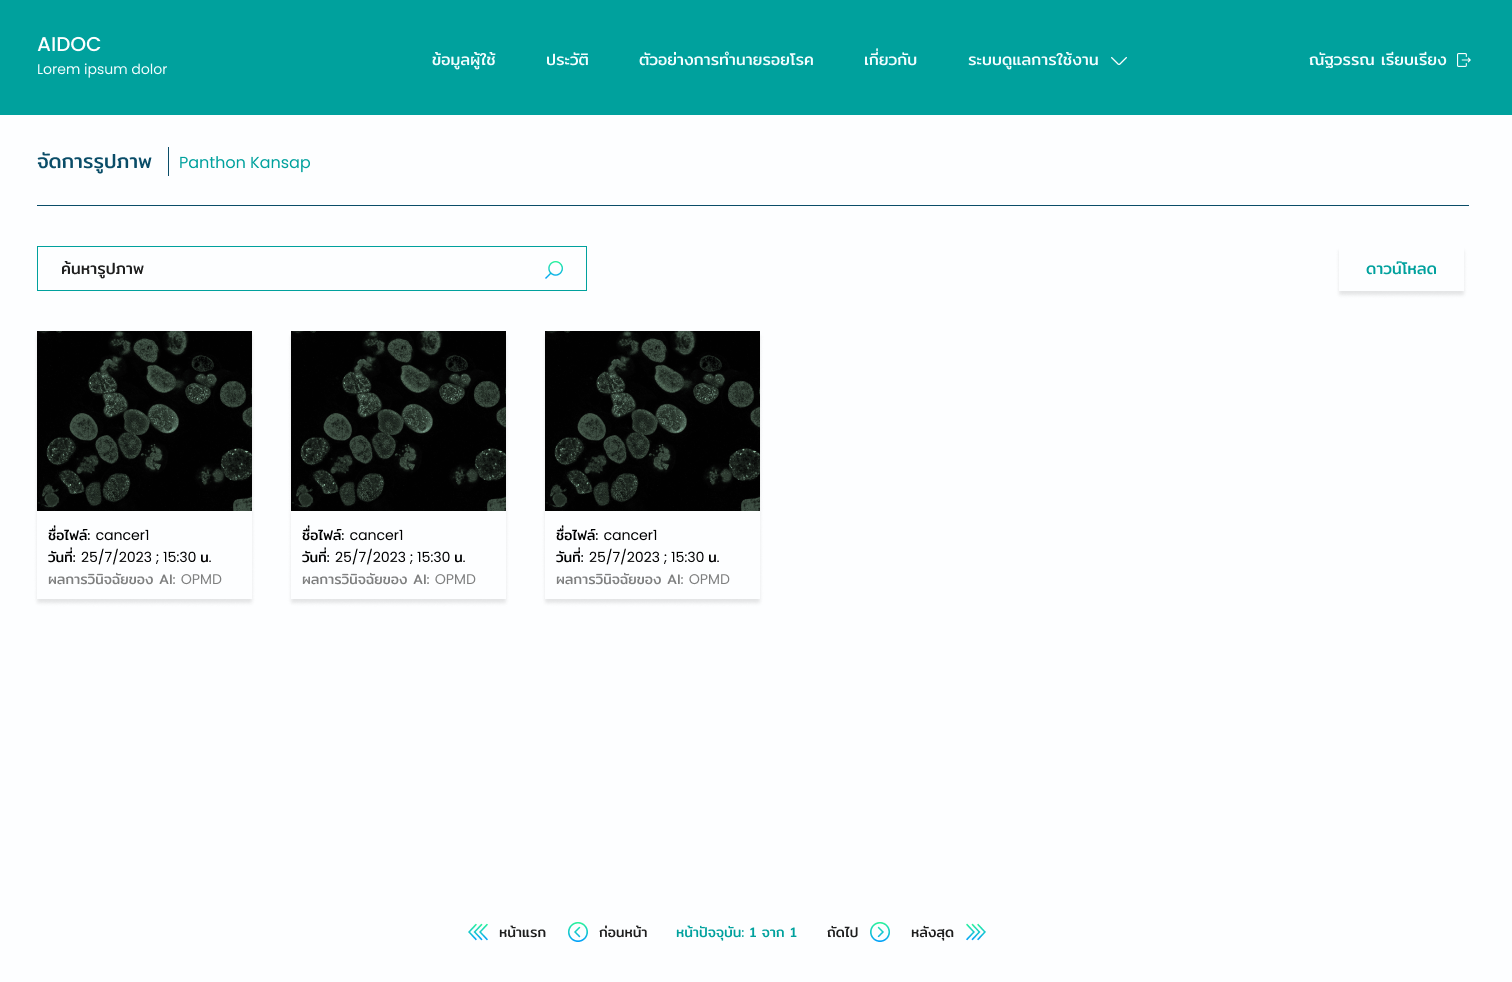
\includegraphics[width=0.7\textwidth]{img/admin/4-admin-image-manamgement-byuser.png}
    \end{center}
    \caption[Poem]{Data Management Page}
    \label{fig:data_management_byuser}
\end{figure}

\newpage
\subsubsection{หน้าจัดการผู้ใช้งาน (User Management Page) โดยแยกตามผู้ใช้งาน}
\begin{figure}[h]
    \begin{center}
        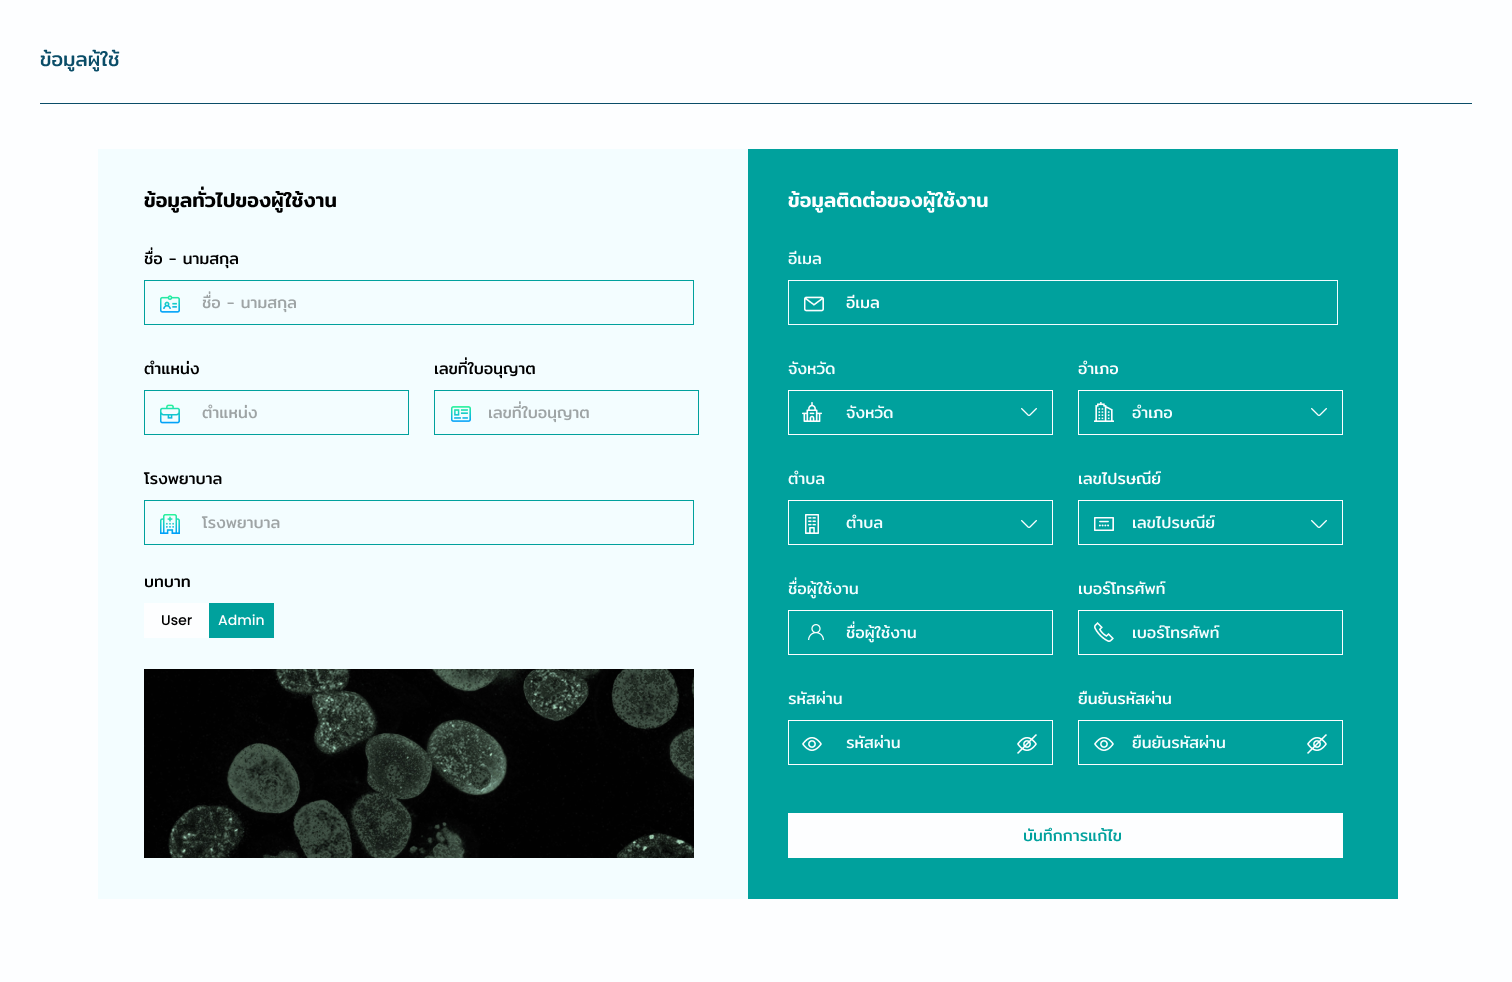
\includegraphics[width=0.7\textwidth]{img/admin/5-admin-edit-user-page.png}
    \end{center}
    \caption[Poem]{Data Management Page}
    \label{fig:data_management_bydisease}
\end{figure}